\subsection{A Common Environment Across Random Arrival Scales}\label{sec:experiment-random}
The third study holds the two reward means fixed before drawing the
arrival schedule. At $T=4^m$, $m=4,5,6,7$, the competing arm has lifetime
$H=4^J$, $J=0,\ldots,m$. We consider probabilities proportional to
$2^{-J}$, uniform scale probabilities, probabilities proportional to
$4^{-J}$, an equal mixture of the last two scales, and a point mass at
the last scale. The anchor mean is $1/2$; the competitor mean is
$1/2\pm\Delta$, with $\Delta=2^{-1-r/2}$, $r=0,\ldots,2m+2$.

One rule starts a fresh two-arm MOSS run with the remaining horizon
revealed by the known endpoint. The other is the original MC-MOSS,
which does not know the endpoint and retains all anchor observations.
Their panels specify this information difference. We simulate the
forced prefix exactly through its binomial sufficient statistic.

For each policy and mixture, we use 64 development replications to
select a single gap and sign, or a separate gap and sign for each lifetime.
Both selections are then evaluated on 128 independent replications per
lifetime. Mixture means use the known schedule probabilities, with
stratified Monte Carlo standard errors. A separate check draws 2048
actual schedules for each selected common environment. These are
held-out risks of development-selected members of a finite grid, not
estimates of the full minimax risk or of a continuous supremum.

Figure~\ref{fig:random-heatmap} shows the conditional risk of a better
arriving competitor. The difficult gap changes with the remaining
lifetime. The retained prefix changes this surface, so the two panels
also differ for reasons beyond endpoint information alone.
Figure~\ref{fig:random-common} then averages over the inverse-square-root
mixture. At the largest endpoint, fresh-horizon MOSS has held-out mean
regret 1.321 (standard error 0.018) under the selected common
environment, compared with 1.977 (0.026) when the selected
environment is allowed to depend on the schedule. The corresponding
geometric values are $W(Q)=1.412$ and $\mathbb E\sqrt H=4.016$.
The latter curve is an arrival-only reference, not an observed risk.

The remaining mixtures, direct schedule draws and selected gaps are
reported in the computational supplement. For the two-long-scale
mixture the held-out ordering is reversed: development selection can
miss the best grid member. Independent evaluation removes reuse of
selection noise from the reported means; it does not make finite-grid
selection exact. None of these finite experiments estimates an
asymptotic rate or establishes that the anytime policy attains the
random-template theorem.

\begin{figure}[tbp]
\centering
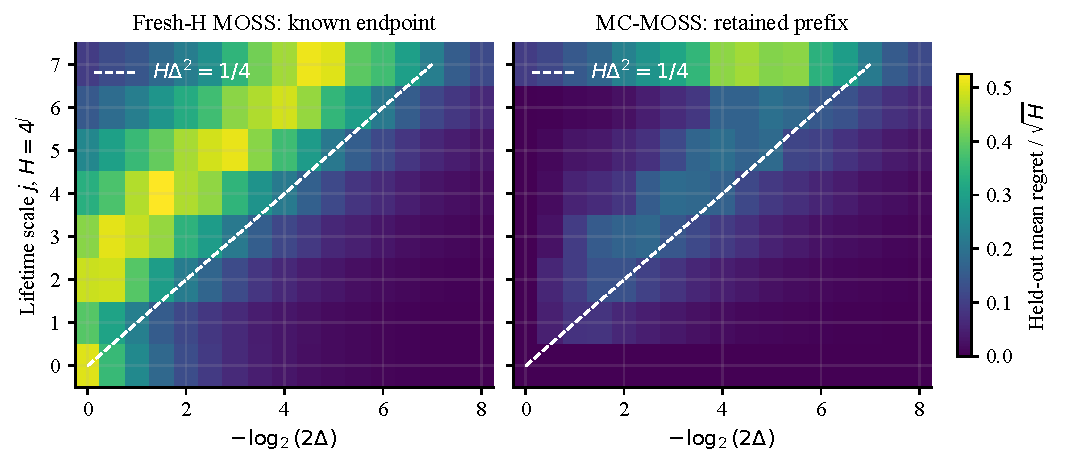
\includegraphics[width=\textwidth]{figures_v2/random_gap_heatmap.pdf}
\caption{Held-out regret divided by $\sqrt H$ for a better arriving
competitor at $T=16384$. Each cell uses 128 replications. The dashed
line marks $H\Delta^2=1/4$; it is a scale reference, not a fitted ridge.
The policies differ in endpoint knowledge and retention of the forced
anchor prefix.}\label{fig:random-heatmap}
\end{figure}
\begin{figure}[tbp]
\centering
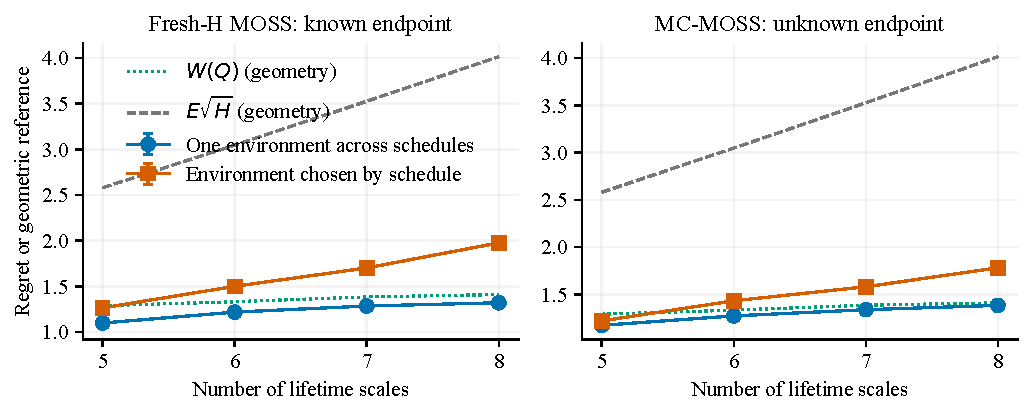
\includegraphics[width=\textwidth]{figures_v2/random_common_gap.pdf}
\caption{Common versus schedule-specific environments under
$\Pr(J=j)\propto2^{-j}$. Environments are selected on development
replications and evaluated independently. Bars are 1.96 stratified
Monte Carlo standard errors. The two geometric reference curves are
computed from the arrival law and are not risk estimates. Selection
is performed separately for each policy; the panels do not compare
the policies under one common mean vector.}
\label{fig:random-common}
\end{figure}
